\documentclass{article}
\usepackage[utf8]{inputenc}
\usepackage[russian]{babel}
\usepackage{graphicx}
\usepackage{amsmath}
\usepackage{wrapfig}
\usepackage{float}

\graphicspath{ {./data/images} }
\author{Александр Романов Б01-107}
\date{}
\title{3.6.1 Спектральный анализ электрических сигналов.}

\begin{document}
\maketitle
\section{Введение}
\subsection{Цель работы}
Изучить спектральный состав периодических электриче­
ских сигналов.
\subsection{В работе используются} 
Анализатор спектра, генератор прямоугольных импульсов и сигналов специальной формы,
осциллограф.

\subsection{Идеи}
\subsubsection{Разложение сложных сигналов в ряд Фурье}

При изучении линейных систем возникает необходимость представления произвольного
сигнла \(f(t)\) в виде ряда Фурье:
\[ f(t) = \sum_n c_ne^{i\omega_nt} \] 

Получим коэффициенты разложения в ряд Фурье для периодического колебательного процесса
общего вида \( f(t) = f(t + T) \), где \( T \) - период процесса. Покажем, что этом случае функция 
\( f(t) \) может быть представленна бесконечной суммой гармонических колебаний с кратными частотами:
\begin{equation} 
    f(t) = \sum_{n=-\infty}^{\infty} c_ne^{in\omega_0t}
    \label{sum_n}
\end{equation}

Нетрудно видеть, что все слогаемые в этой сумме -- периодические функции с периодом, кратным \(T\) и они
полностью исчерпывают набор гармонических функций, удовлетворяющих \( f(t) = f(t + T) \). Таким образом 
периодическая функция имеет дискретный спектр с кратными частотами.
Спектр -- то есть набор коэффициентов \(\{c_n\}\) -- можно найти следующим образом: домножим обе части
равенста (\ref{sum_n}) на \( e^{-im\omega_0t} \) и проинтегрируем по времени \(t\) за период (Например, от 0
до \(T\)). Получим

\begin{equation*}
    \int_0^T f(t)e^{-im\omega_0t}dt  \sum_n c_n \int_0^T e^{i(n - m)\omega_0t}dt
\end{equation*}

Вычислим интеграл в правой части:

\begin{equation*}
    \int_0^T e^{i(n-m)\omega_0t}dt = 
    \begin{cases}
        0 \quad if \: n \neq m\\
        T \quad if \: n = m\\
    \end{cases}
\end{equation*}

Таким образом получаем

\begin{equation}
    c_n = \frac{1}{T}\int_0^T f(t)e^{-in\omega_0t}dt.
    \label{cn}
\end{equation}

\subsubsection{Периодическая последовательность прямоугольных импульсов}


\begin{figure}[H]
\centering
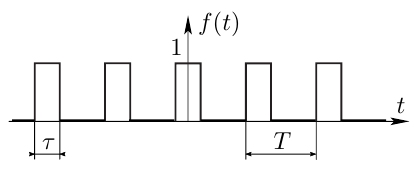
\includegraphics[width=0.5\textwidth]{sq_imp_example.png}
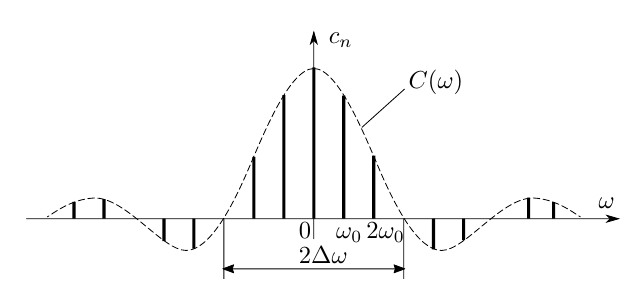
\includegraphics[width=0.5\textwidth]{sq_imp_spect_example.png}
\caption{Периодическая последовательность прямоугольных импульсов и её спектр(Для $\tau = \frac{T}{3}$).} 
\label{sq_imp_example}
\end{figure}
Рассмотрим сигнал на рис \ref{sq_imp_example}
.


\subsubsection{Периодическая последовательность цугов гармонических колебаний}

\begin{figure}[H]
    \centering
    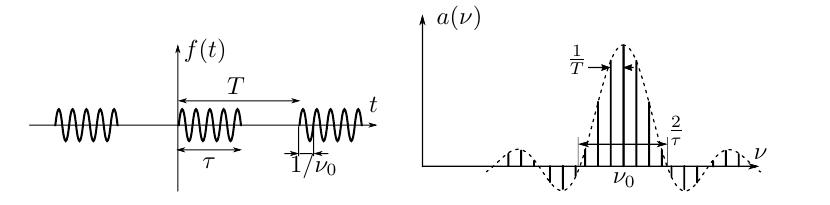
\includegraphics[width=\textwidth]{cug_imp_example.png}
    \caption{Периодическая последовательность прямоугольных импульсов и её спектр.} 
    \label{cug_imp_example}
\end{figure}

Рассмотрим сигнал на рис \ref{cug_imp_example}. Это - цуги колебания \( A_0 \sin \left(\nu_0t\right) \)
Снова пусть $T$ кратно $\tau$. Тогда Спектры последовательности идентичны прямоугольным импульсам, но
сдвинуты на $\nu_0$. Соотношения неопределённости остаются прежними:

\[ \Delta\nu\tau \simeq 1 \]
\[ \delta\nu T \simeq 1 \]

\subsubsection{Амплитудно-модулированные колебания}
\begin{figure}[H]
    \centering
    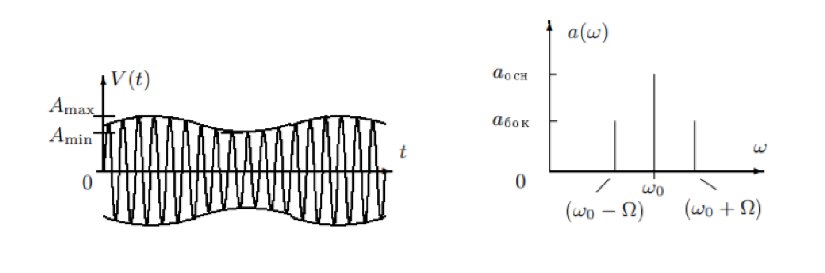
\includegraphics[width=\textwidth]{AM_signal_example.png}
    \caption{Амплитудно-модулированный сигнал и его спектр.} 
    \label{AM_sig_example}
\end{figure}

Рассмотрим (Рис. \ref{AM_sig_example}) гармонические колебания высокой частоты $\omega_0$, амплитуда которых
медленно меняется по гармоническому закону с частотой $\Omega \ll \omega$.

\[ s(t) = A_0\left[1 + m \cos \Omega t\right] \cos \omega_0 t \]

Коэффициент $m$ называется \emph{глубиной модуляции}. При \( m < 1 \) амплитуда меняется от минимальной 
\( A_{min} = A_0(1 - m) \) до максимальной \( A_{max} = A_0(1 + m) \). Глубина модуляции может быть представленна
в виде

\[ m = \frac{A_{max} - A{min}}{A_{max} + A_{min}}. \]

Отсюда можно легко переписать уравнение сигнала как:

\[ s(t) = A_0 \cos \omega_0t + \frac{A_0m}{2} \cos \left(\omega_0 + \Omega\right)t  + \frac{A_0m}{2} 
\cos \left(\omega_0 + \Omega\right)t.\]

\section{Работа}

\subsection{Исследование спектра периодической последовательности прямоугольных импульсов}

Устанавливаем на генераторе прямоугольные импульсы с \( \nu_{rep} = 1kHz \) и длительностью импульса
\( \tau = 100uS \). Получаем на экране спектр сигнала и, изменяя поочереди $\tau$ и $\nu_{rep}$ будем
наблюдать как изменяется спектр.

\begin{figure}[H]
    \centering
    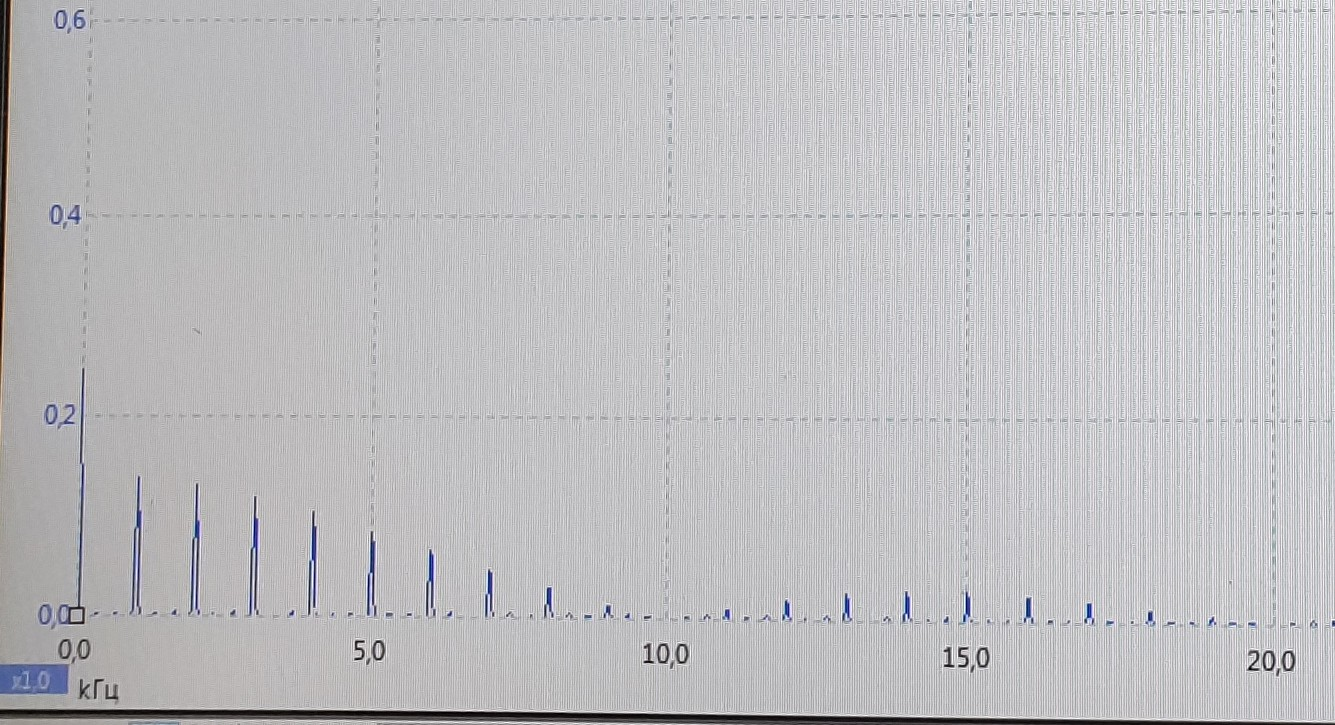
\includegraphics[width=0.6\textwidth]{1.jpg}
    \caption{Спектр при \( \nu_{rep} = 1 kHz, \tau = 100uS \)}
    \label{spec_1}
\end{figure}

\begin{figure}[H]
    \centering
    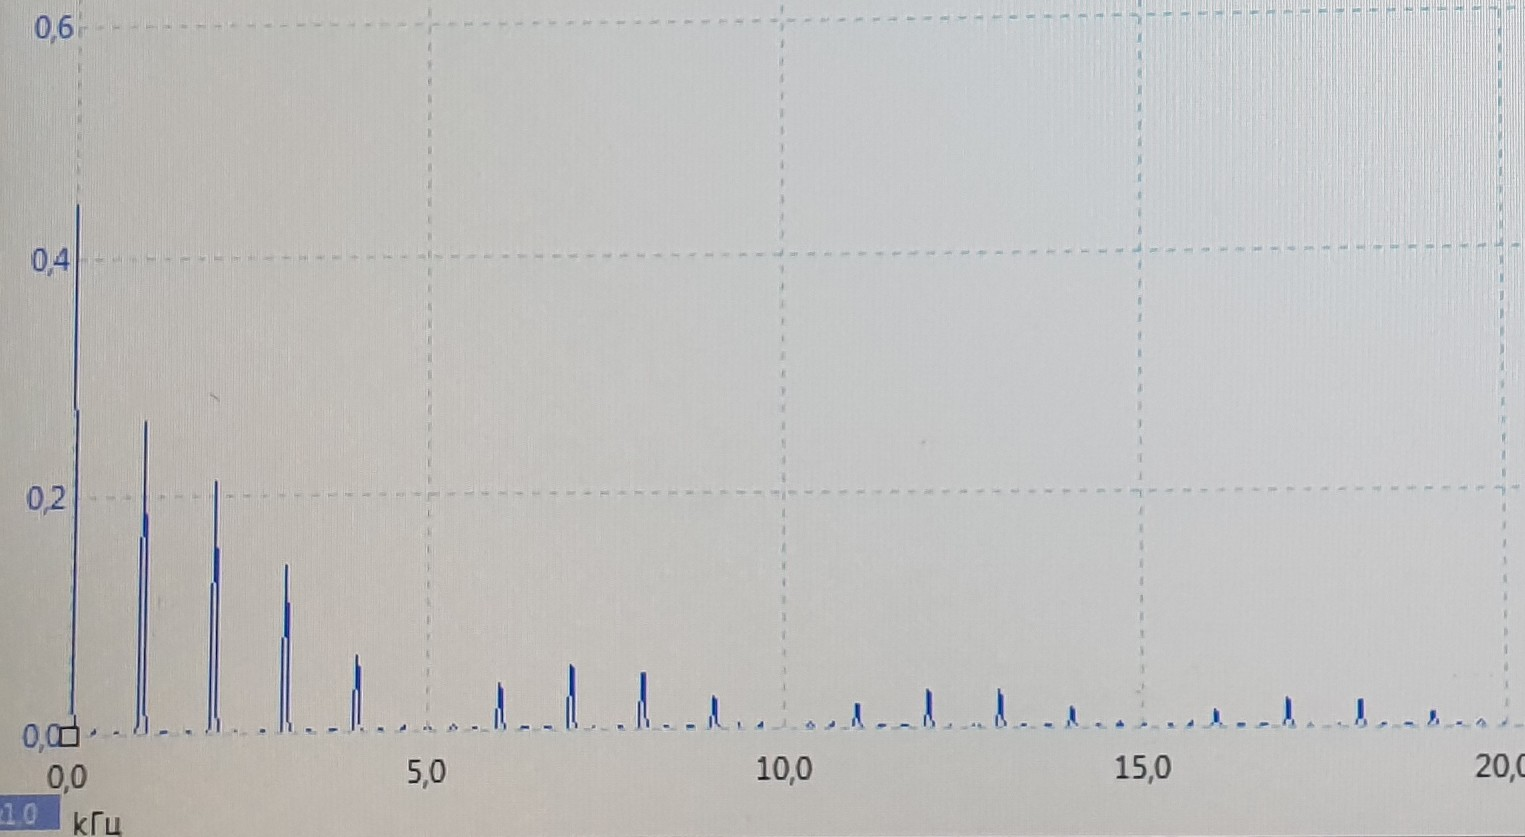
\includegraphics[width=0.6\textwidth]{2.jpg}
    \caption{Спектр при \( \nu_{rep} = 1 kHz, \tau = 200uS \)} 
    \label{spec_2}
\end{figure}

\begin{figure}[H]
    \centering
    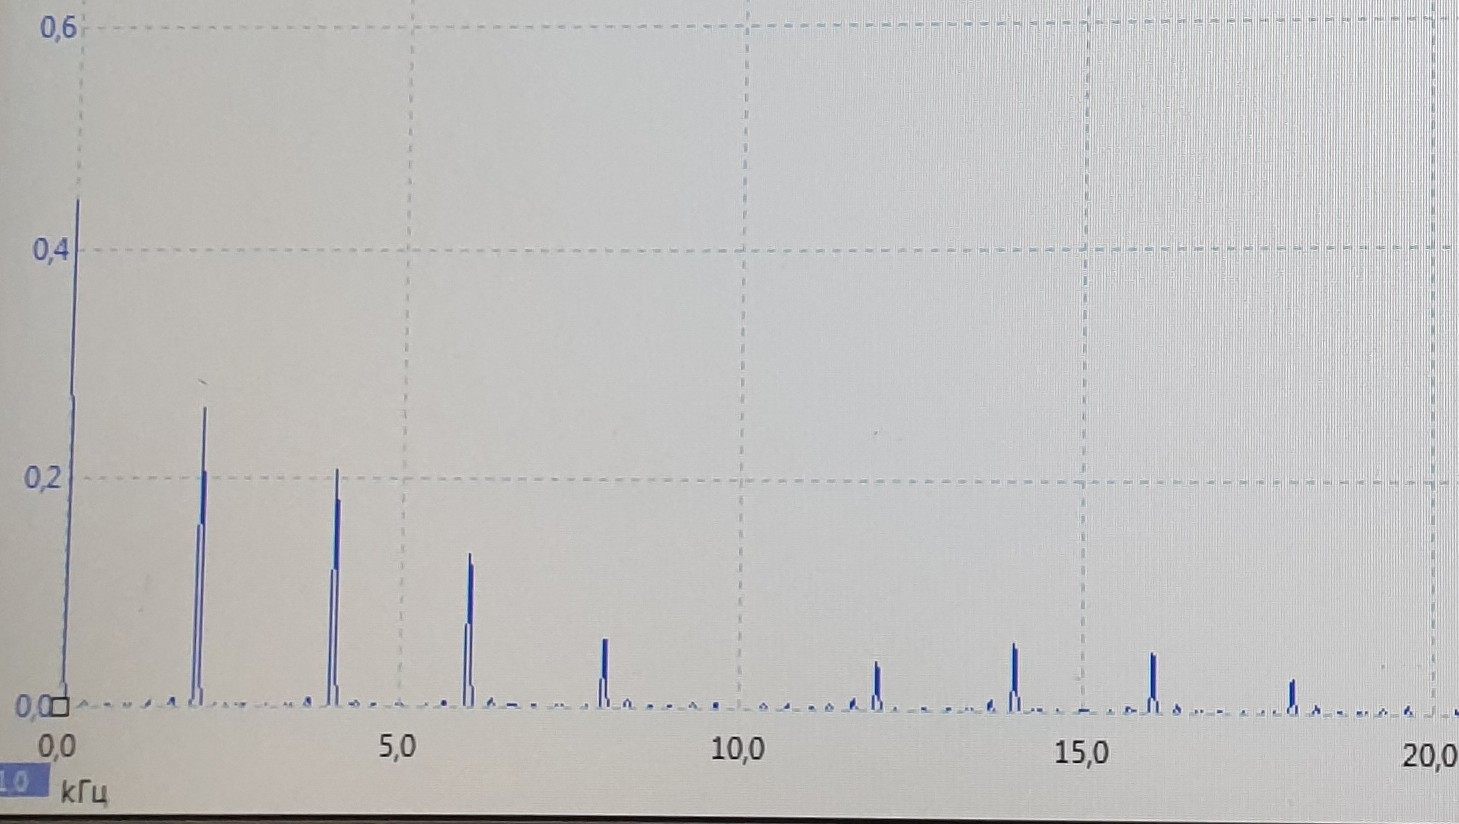
\includegraphics[width=0.6\textwidth]{3.jpg}
    \caption{Спектр при \( \nu_{rep} = 2 kHz, \tau = 100uS \)} 
    \label{spec_3}
\end{figure}


\section{Выводы}
\end{document}